\documentclass[conference]{IEEEtran}

\usepackage[T1]{fontenc}
\usepackage[utf8]{inputenc}
\usepackage[french]{babel}
\usepackage{array}
\usepackage{booktabs}
\usepackage{graphicx}
\usepackage{url}

\title{Examen Machine OS202}

\author{
\IEEEauthorblockN{Santiago Florido Gomez}
\IEEEauthorblockA{
Ing\'enieur m\'ecatronique\\
\'Etudiant STIC, ENSTA Paris
}
}

\begin{document}

\maketitle

\begin{abstract}
Ce document, r\'edig\'e au format IEEE, pr\'esente une synth\`ese de l'environnement
mat\'eriel observ\'e depuis WSL pour les travaux du module OS202. Les informations
ont \'et\'e obtenues \`a l'aide de la commande \texttt{lscpu} et sont reformul\'ees
sous forme de tableaux en fran\c{c}ais.
\end{abstract}

\section{Caract\'eristiques de l'environnement}

Le Tableau~\ref{tab:cpu-general} regroupe les informations g\'en\'erales sur
l'architecture processeur visibles depuis WSL.

\begin{table}[!t]
\caption{Informations g\'en\'erales du processeur}
\label{tab:cpu-general}
\centering
\small
\begin{tabular}{p{0.43\columnwidth} p{0.47\columnwidth}}
\toprule
\textbf{Champ} & \textbf{Valeur} \\
\midrule
Architecture & x86\_64 \\
Modes d'op\'eration CPU & 32-bit, 64-bit \\
Tailles d'adressage & 46 bits physiques, 48 bits virtuels \\
Ordre des octets & Little Endian \\
Nombre de CPU logiques & 16 \\
Liste des CPU en ligne & 0-15 \\
Identifiant du fabricant & GenuineIntel \\
Nom du mod\`ele & Intel(R) Core(TM) Ultra 7 155H \\
Famille CPU & 6 \\
Mod\`ele & 170 \\
Threads par coeur & 2 \\
Coeurs par socket & 8 \\
Sockets & 1 \\
Stepping & 4 \\
BogoMIPS & 5990.39 \\
Virtualisation & VT-x \\
Fournisseur de l'hyperviseur & Microsoft \\
Type de virtualisation & full \\
\bottomrule
\end{tabular}
\end{table}

Le Tableau~\ref{tab:cpu-cache} pr\'esente les informations de cache et
d'organisation NUMA disponibles dans la m\^eme sortie \texttt{lscpu}.

\begin{table}[!t]
\caption{Caches et topologie m\'emoire}
\label{tab:cpu-cache}
\centering
\small
\begin{tabular}{p{0.43\columnwidth} p{0.47\columnwidth}}
\toprule
\textbf{Champ} & \textbf{Valeur} \\
\midrule
Cache L1d & 384 KiB (8 instances) \\
Cache L1i & 512 KiB (8 instances) \\
Cache L2 & 16 MiB (8 instances) \\
Cache L3 & 24 MiB (1 instance) \\
Nombre de noeuds NUMA & 1 \\
CPU du noeud NUMA 0 & 0-15 \\
\bottomrule
\end{tabular}
\end{table}

Ces valeurs ont \'et\'e mesur\'ees directement depuis WSL. Elles diff\`erent donc
d'une configuration \`a l'autre selon la machine h\^ote et les ressources
allou\'ees \`a l'environnement virtuel.

\section{Question préliminaire}
Il n'est pas représentatif, car la galaxie, dans une première approximation de simulation, peut être identifiée à une forme de disque plan qui ne présente pas une distribution considérable dans la direction \(Oz\). C'est justement cette condition de concentration sur l'axe \(z\) qui fait que l'implémentation de davantage de couches en \(N_k\) conduise à une complication considérable de la grille et de la distribution des éléments dans la grille, sans que l'approximation faite du système ne soit améliorée de manière significative.


\section{Section a paralelizer}
Pour l’évaluation du temps que représente chacune des étapes de la simulation, il est proposé de mesurer les temps. À chaque itération, un temps est pris avant et après le rendu, ainsi qu’un autre avant et après la mise à jour de la simulation, en utilisant \texttt{time.perf\_counter()}. Ces mesures sont prises à chaque frame, puis le temps consommé est moyenné toutes les 60 frames. Les résultats

\begin{verbatim}
[timing] 60 frames mesurées | avg_render=3.325 ms | avg_update=163.532 ms
[timing] 120 frames mesurées | avg_render=3.344 ms | avg_update=165.161 ms
\end{verbatim}

montrent que la partie dominante du code se trouve dans le temps de mise à jour (\textit{update}), qui inclut les calculs des accélérations ainsi que les mises à jour des positions et des vitesses. Étant donné qu’il s’agit de la section dominante de la simulation, on considère que la section de calcul et de mise à jour des corps à l’intérieur de la grille est la plus susceptible d’être parallélisée.
\section{Shared memory paralelization avec numba}

Étant donné que Numba est une méthode d’implémentation de la parallélisation en mémoire partagée, ce qui est proposé est de remplacer par \texttt{prange} les boucles dans lesquelles chacune des itérations correspond au résultat d’un corps distinct et qui écrivent dans des positions éloignées du tableau, afin d’éviter des phénomènes comme les blocages dus à la synchronisation, qui pourraient affecter la qualité des résultats de la parallélisation initiale. En suivant cette idée, il est proposé d’implémenter la parallélisation avec mémoire partagée (\textit{Numba}) pour le calcul en plusieurs threads de l’accélération des corps ; pour cela, le décorateur est défini à \texttt{true} et, en outre, \texttt{range} est remplacé par \texttt{prange}. La parallélisation avec mémoire partagée n’est pas implémentée dans le calcul de la grille, car la présence de structures qui sont partagées, comme c’est le cas de \texttt{cell\_counts}, \texttt{current\_counts} et \texttt{body\_indices}, pourrait donner lieu à des problèmes de synchronisation dans la mémoire partagée et à une dégradation des résultats du calcul.

\begin{figure}[htbp]
\centering
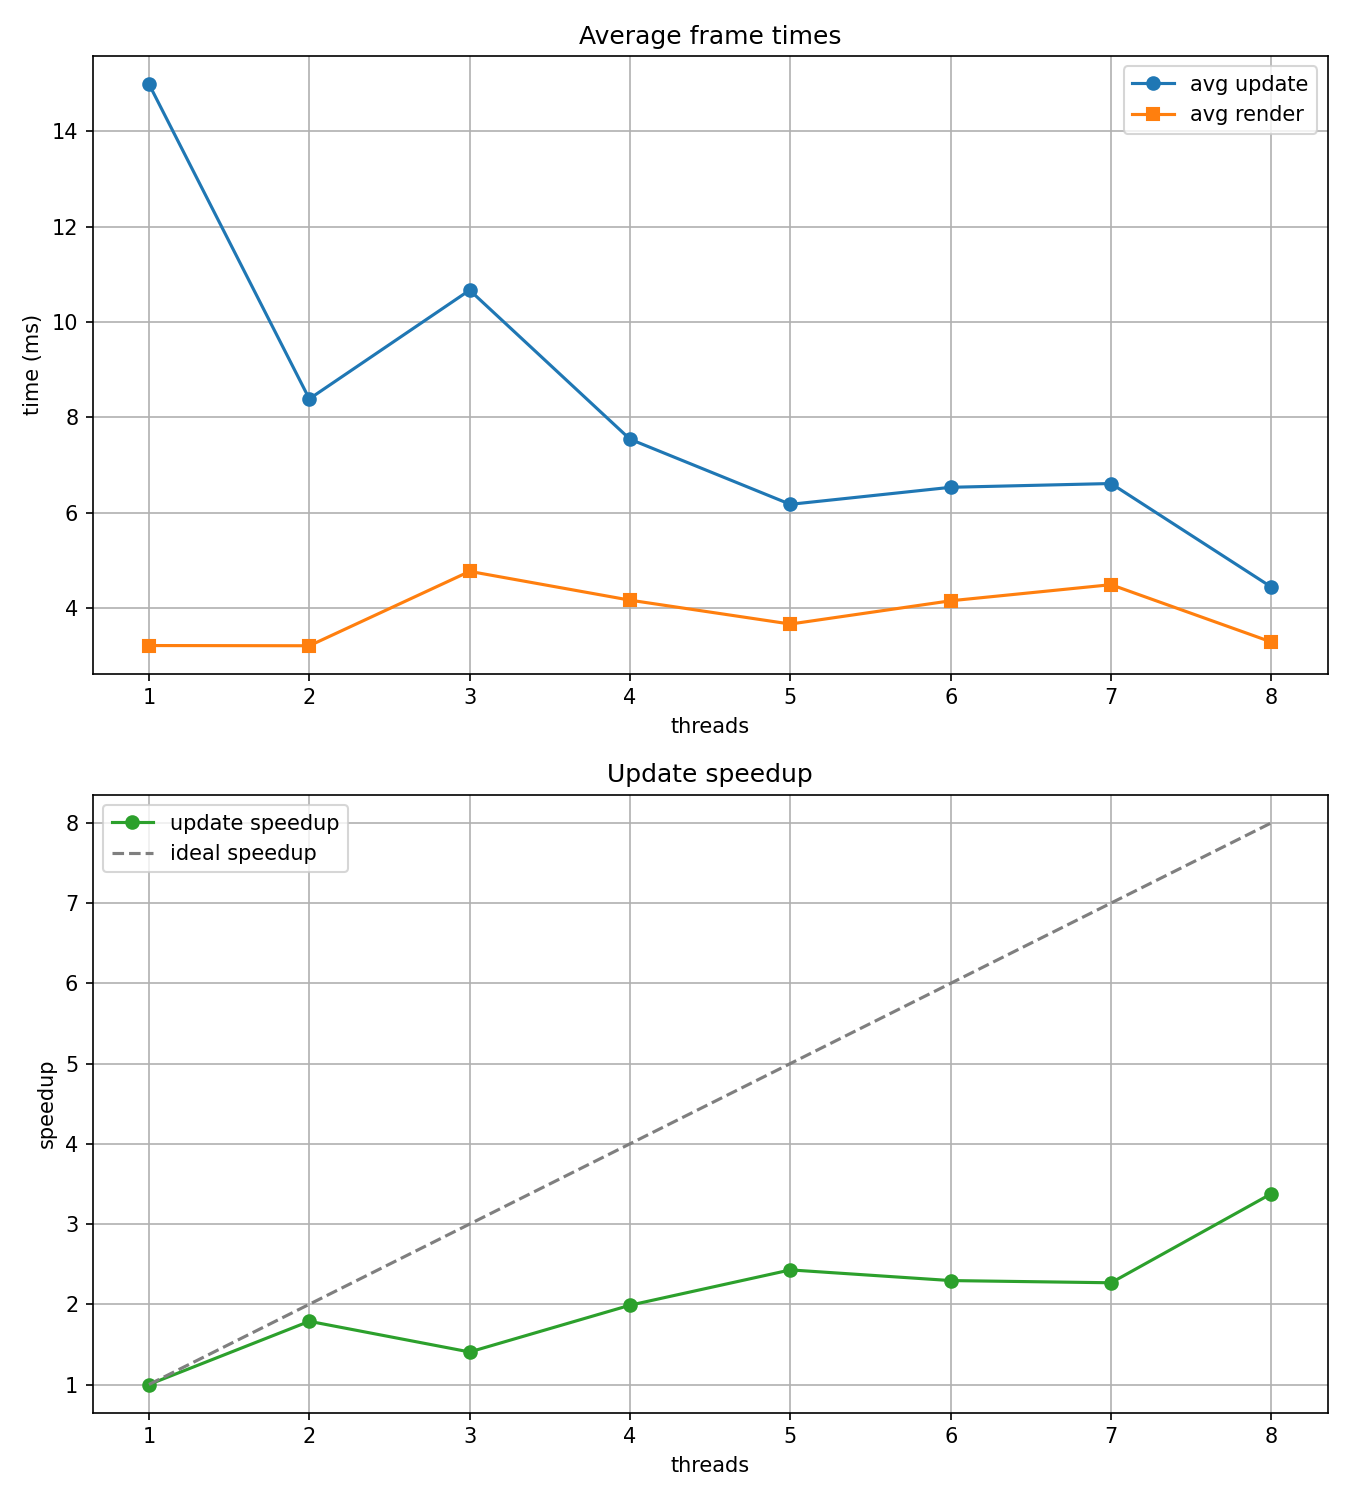
\includegraphics[width=\linewidth]{images/numba_parallel_timings.png}
\caption{Temps moyens de rendu et de mise à jour, ainsi que l’accélération obtenue en fonction du nombre de threads Numba.}
\label{fig:numba_parallel_timings}
\end{figure}


Les résultats montrent la diminution du temps moyen de rendu à mesure que l’on augmente le nombre de threads de calcul dans lesquels est répartie la boucle principale pour l’accélération de chaque corps. Néanmoins, on peut constater que le degré d’amélioration du temps de traitement à partir du deuxième thread s’éloigne du \textit{speedup} idéal, ce qui peut être lié aux effets de synchronisation de la mémoire partagée, aux limitations imposées par les sections du code qui ne sont pas parallélisables, ou encore au fait que la dynamique de la grille n’a pas été modifiée en utilisant Numba, étant donné que la nature de ses accès mémoire ne la rendait pas idéale pour cette implémentation.
\end{document}
